\chapter{Architectural description} \label{chap:ArchitecturalDescription}

This chapter will first present the data model for the system, then move on to show the overall architecture of the system: Which client applications there are, how they communicate with the server and external APIs, and how the server communicates with the database. The chapter will then look closer on each of the components, the backend, Android and iOS application, and show what the architecture within each of these looks like. 
\section{Data model}
The system is oriented around the following entities:
\begin{description}
    \item{User: } \\
        A user represents a user of the system. It has a name, a username that is used to identify him in the system, a e-mail address, a unique \gls{ID}-number in the database to identify him uniquely within other data, and a password. The password is hashed using bcrypt. \cite{bcrypt}
    \item{Book: } \\ 
        A book is identifies a user owning a specific book with a specific \gls{ISBN}. The book is saved to the database with the fields ''owner'', ''isbn'', ''googleid'', ''rentedTo'' and ''availableForRent''. Both ''owner'' and ''rentedTo'' are \gls{ID}-numbers that are used to identify the user owning and loaning in the User-database. The field ''rentedTo'' is set to null if no one is loaning the book. The field ''availableForRent'' tells us if the owner allows people to loan the boook.
    \item{Crowd: } \\ 
        A crowd, which is called a group in the \gls{UI} in the last versions of the mobile applications, captures the social aspect of CrowdShelf. A crowd has a ''name'', ''owner'' and a list of ''members''. The two last fields, ''owner'' and ''members'', operate on \gls{ID}-numbers from the user-database. 
\end{description}

The data is saved in a \gls{DBMS} called MongoDB. \cite{mongodb} MongoDB saves data as \gls{BSON}, which is based on \gls{JSON}, which is used as the data format for sending data between the server application and the mobile applications. \cite{bson}

\section{System architecture}
The complete system has a server application which talks to a database system. The team developed two mobile applications, one for Android and one for iOS. The application architecture is based on the \gls{MVC} pattern, see section \ref{arch:mvc} The relationship between the client applications and the \gls{backend} is oriented around the simple client-server architectural pattern. \cite[p.217-219]{progark} The complete system developed by the team is following the architectural pattern called the ''layered pattern''. \cite[p. 205-210]{progark}. The server application can be seen as a layer that talks to two other layers: The database and the client applications. All database communication from the client applications goes through the server application.  In addition, both mobile applications talked to an external \gls{API} from Google\cite{google-books-api}, which means the system also utilizes the service-oriented architectural pattern. \cite[p. 222-226]{progark} The Google Books \gls{API} is used to fetch meta information about the books. The use of external services can be extended if the need for data demands it. 

For an overview of the complete system architecture, see figure \ref{fig:system-arch-final-simple}.

\begin{figure}
    \begin{center}
        \includegraphics[width=10cm,keepaspectratio]{figs/system-arch-final-simple.png}
        \caption{Diagram that shows the components in the complete system, and how they communicate.}
        \label{fig:system-arch-final-simple}
    \end{center}
\end{figure}



\subsection{\gls{MVC} in the client applications}
\label{arch:mvc}
Both mobile applications in the the system are based on the \gls{MVC} pattern. This is an architectural pattern that tries to solve problems related to multiple views trying to update and read the same data. \cite[p. 212-215]{progark} The pattern is based around the idea that logic, views and data should be separated. The model contains data and methods related to operations on the data. The view controls how the data is presented to the user in the \gls{UI}. The view controller is used to manage user interaction, and send messages to the views and models when updates are needed. The relationshp between these groups of modules, the controllers, models and views, is illustrated in figure \ref{fig:mvc}. 

\begin{figure}
    \begin{center}
        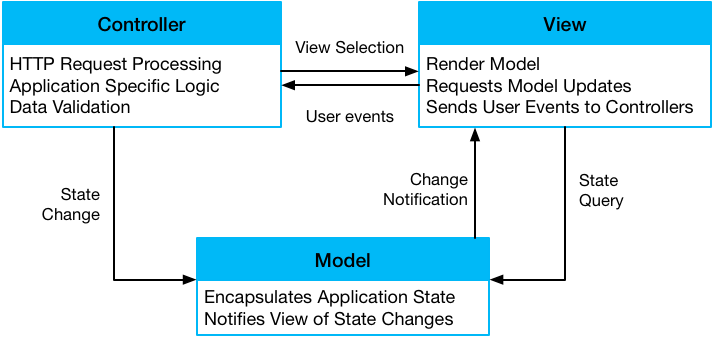
\includegraphics[width=10cm,keepaspectratio]{figs/mvc.png}
        \caption{Diagram that shows how the components of the \gls{MVC} pattern interact.}
        \label{fig:mvc}
    \end{center}
\end{figure}

\section{Backend}
The server application is written in Node with the Express framework, and is structured with \gls{MVC}, but without the views. \cite{nodejs}\cite{express}\cite[p.~432]{software-engineering}. Based on two layers, the controllers and the models, together with a specific controller, the \code{tokenController} which checks that a user is authorized, and the actual \gls{API} that connects routes to controller methods, the server application is based on the layered architectural pattern. See figure \ref{fig:server-detail}. It is important that each layer only communicates with the layer above or below.


\begin{figure}
    \begin{center}
        \includegraphics[width=10cm,keepaspectratio]{figs/arch-server-detail.png}
        \caption{Diagram that shows how the layers in the server application communicate with each other, and the database.}
        \label{fig:server-detail}
    \end{center}
\end{figure}

\subsection{System structure}
Node is oriented around so called modules, where methods available to other modules are exported. This section will go through the modules, that is each file as one file is one module, and explain how it fits into things. It has the following file structure, where each file is a module:
\begin{description}
    \item{\textbf{\code{models/}}} This folder contains models, and methods for handling data and communication with the database.
        \begin{description}
            \item{\code{user.js}, \code{book.js} and \code{crowd.js}} \\ 
                Each of the connects to the database and maintains a connection to it. Exports methods for different queries for the entity, update and inserts. 
            \item{\code{token.js}} \\ 
                This module is used to generate tokens, and see if they are valid. The tokens are used for authorization when requesting resources. The point her is that users that are not registered should not be allowed to neither add or remove data from our databases. The module exports two methods: \code{generate} and \code{isValid}. The \code{generate}-method uses the external library ''hat'' to give a random string. \cite{hat} It alos gives it an expiration date, which is 20 minutes ahead in tme. It then adds that token with the expiration date to the database. The  \code{isValid}-method looks up a given token to see if it is still valid. This is used by the \code{tokenController.js}-module every time the user tries to do a request.
            \item{\code{forgottenPasswordKeys.js}} \\
                This module works the same way as token, but is used when users have forgotten their password. It generates a number of 5 ciphers, then adds it to the database with a 20 minute expiration. The  \code{forgottenPasswordController.js} -module uses the \code{isValid}-method to see if a entered key is valid.
        \end{description}
    \item{\textbf{\code{controllers/}}} Has the controller-modules, which handles the requests from the client. 
        \begin{description}
            \item{\code{userController.js}, \code{bookController.js} and \code{crowdController.js}} \\ 
                Each of the controllers export methods for handlign requests from the clients. These are connected with the actual routes and \gls{HTTP}-methods by the ''setup''method in the router-module. The controllers have all logic for these entities. They work towards their respective model-modules for handling data operations.
            \item{\code{passwordController.js}} \\ 
                The \code{passwordController}-module has all the logic for passwords. The passwords themselves are saved with the \code{user}-object, but this controller has methods for hashing a clear text password, and checking if a given hash is the same as a clear text password. The hashing mechanisms utilize an external library built around the bcrypt-algorithm. \cite{bcrypt} The module exports the two methods \code{hash} and \code{isValid}.
            \item{\code{tokenController.js}} \\
                The \code{tokenController} has the logic for the authentication features. When a user logs in a middleware-method in this controller is called. The method checks if the requested \gls{URL} is protected. If it is, it requires a token. If the client gave a token, and it is valid, then the \code{tokenController} lets the request go through. If not, it returns an error message. 
            \item{\code{emailController.js}} \\
                Contains a e-mail method for each of the e-mails that can be sent, that is one for inviting a user, one for resetting a password and one welcome e-mail for a user that just registred. These methods use the helpers to put the e-mail together. That is they get the data needed by the callee, for instance reciepents e-mail addres and name, use that to render the content and then send the e-mail. 
        \end{description}
    \item{\textbf{\code{helpers/}}} This folder contains modules that help and assist the controller, but does not handle requests themselves.
        \begin{description}
            \item{\code{emailSendingHelper.js}} \\ 
                This helper-module exports a method for sending an e-mail to one or more users. It initializes by using environment variables to define which \gls{SMTP}-server to use, then exports a method to send e-mails with. The method takes recipient, subject, content and a callback-method. This helper is used by the e-mail controller for actually sending e-mails.
            \item{\code{emailTemplateHelper.js}} \\
                Simply used to build e-mail content. It has a build-method that takes the template to be used, the content to be entered and a callback-method. This can be used by the e-mail controller to build an e-mail.
            \item{\code{standardResponsens.js}} \\
                This helper contains some standard responses. This means that the controllers can go her for standardized responses, for example for a ''404 Not found''-response, or ''401 Unauthorized''. This gives the development team one place to change responses that are used across the application.
        \end{description}
    \item{\textbf{\code{emailTemplates/}}} Holds folders for each of the templates, ''inviteUser'', ''registerNewUser'' and ''resetPassword''. Each folder contains two files, one for rendering a HTML-output, and one for a clear text output.
    \item{\textbf{\code{router.js}}} This module sets up all the routes, and which methods to call when a request comes in on that route. 
    \item{\textbf{\code{server.js}}} The server-module has a simple start-method, that calls the router and defines which port to listen to.
    \item{\textbf{\code{index.js}}} The index-module is an entry point for the server, if you want to run it locally. The reason that the server-module in itself does not start the server, is that one does not know how other other applications wants to use this one. This means that any other application can start any number of servers by using the server-module. To run a single local server, the index-module is the entry point. 
\end{description}

There's also a \code{public}-folder that holds the SwaggerUI, which is served by the API-layer on \url{/api}.\cite{swagger-ui}

\section{Android}
\label{architecture-android}
The Android application is developed as an native application using the programming language Java and the \gls{IDE} Android Studio.\cite{android-studios} The application is based on the \gls{MVC}-pattern. It is based around the Android application component called \code{Activity}, which is a part of the Android development environment. These activities work as both the views and the controllers in the application. The application also uses the publish-subscribe pattern \cite[p. 226-229]{progark} through the Otto event bus, to update the views with data received from the models. \cite{otto}

\subsection{User interface structure}
Figure \ref{fig:AndroidUIClassDiagram} shows how the \gls{UI} of the application is structured. The blue squares in figure \ref{fig:AndroidUIClassDiagram} illustrates activities, the green squares illustrates fragments while the grey boxes illustrates classes used for interaction with the models. An activity can start another activity by using an intent.\cite{android-intent} An intent describes and operation to be performed such as starting an activity. All activities in the application is started using intents. 

\subsubsection{Activities}
    An activity is a screen with which the user can interact.\cite{android-activity} In the \gls{MVC} pattern, activities works as both views and controllers. The \code{MainTabbedActivity} activity in figure \ref{fig:AndroidUIClassDiagram} is initially started when the application launches, this activity also contains multiple fragments. It is this activity that both requests data from the \code{MainController.java} class and subscribes to events using the publish-subscribe pattern \cite[p. 226-229]{progark}. Making it able to both manipulate and receive data.
    
\subsubsection{Fragments}
    A fragment consists only in the context of an activity and often has a small function in the user interface of the application.\cite{android-fragment} A fragment can contain multiple fragments, but all the fragments are controlled by the activity containing the outermost fragment. For instance the fragment \code{BookGridViewFragment} in this application is used to show a list of books and notify the \code{MainTabbedActivity} if a book is clicked on. 

\begin{figure}
    \centering
    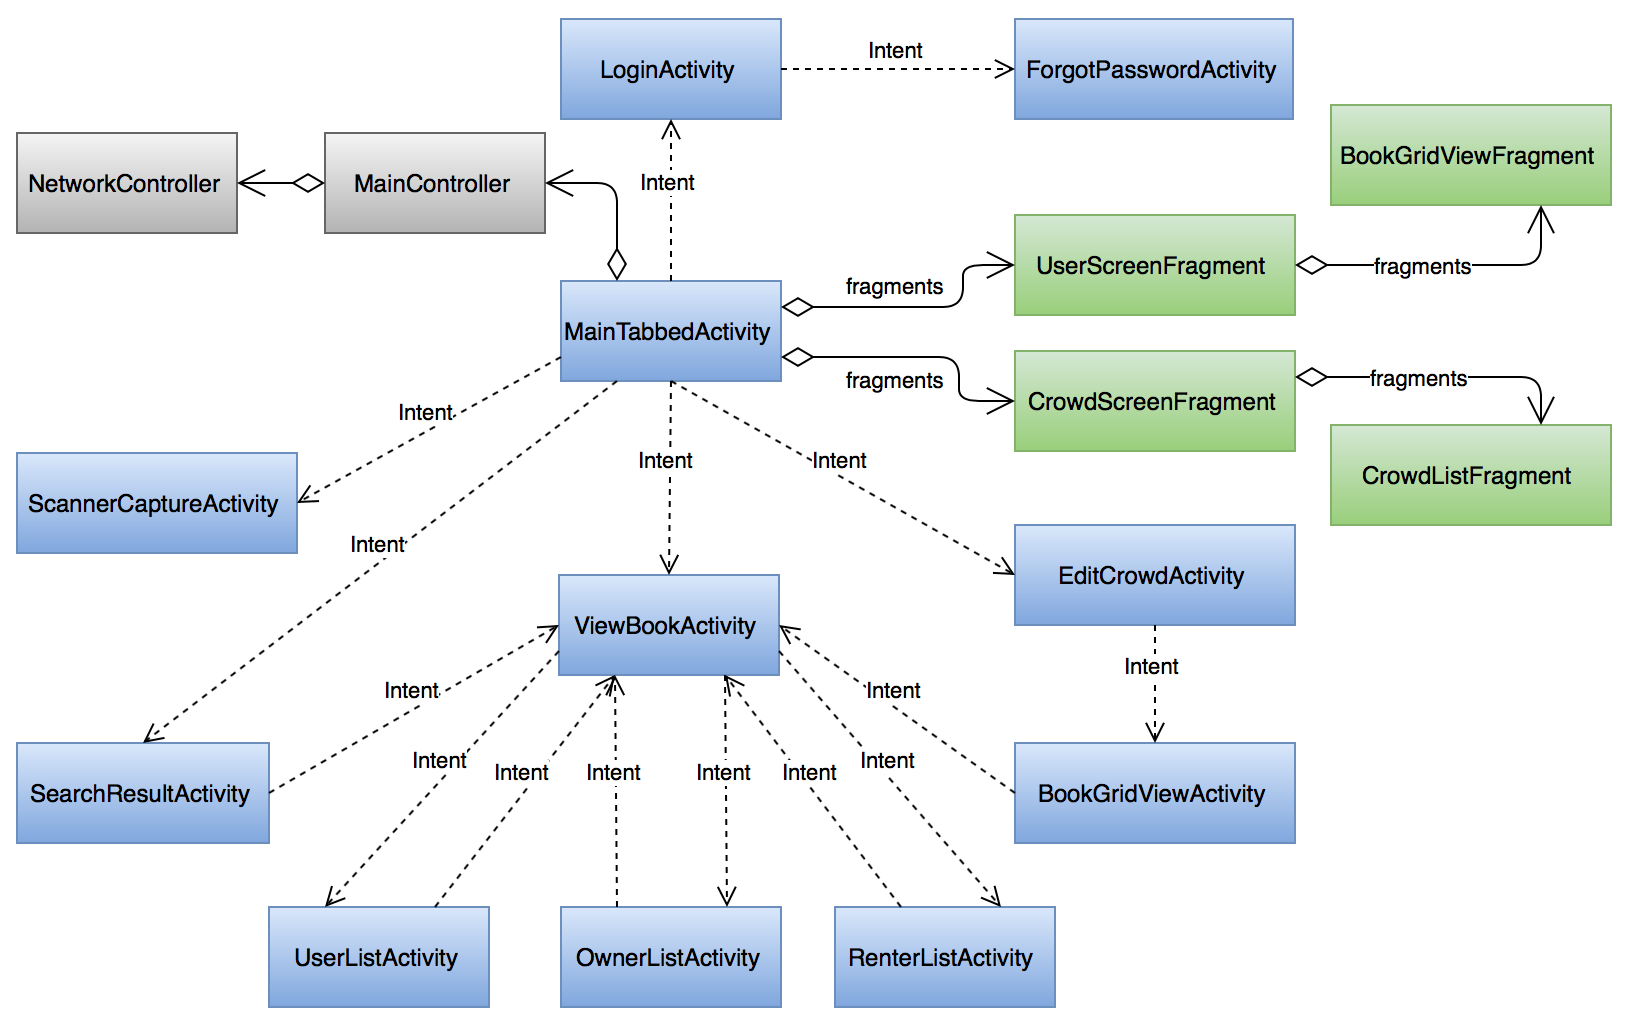
\includegraphics[width=\textwidth,keepaspectratio,origin=c]{figs/v06/Android/AndroidUIClassDiagram.png}
    \caption{Class diagram for UI in Android application version 0.6}
    \label{fig:AndroidUIClassDiagram}
\end{figure}

\subsection{Network, API and storage}
When a view wants to display some information, like the books of a user, or modify some objects, like creating a user, it calls a corresponding method in the \code{MainController}-class. The \code{MainController} will update the local database, if necessary, before calling the \code{NetworkController} which formulates the request to conform to the library service \gls{API}. The \code{NetworkController} has methods for each of the \gls{API} functions, such as retrieving a book, and the methods will concoct a request with an URI and JSON-data to be sent to the backend. In addition, each method might specify a reponsehandler \textemdash  the class that handles the response from the backend. The \code{NetworkController} then forwards the request to the  \code{NetworkHelper} which sends the request to the backend, retrieves the response and forwards the response to the responsehandler. 

There are responsehandlers for each object model: user, crowd, book, in addition to lists containing multiple of the aforementioned objects. The responshandlers converts the response from the backend, which is in JSON-format, to Java-objects and stores or updates the object in the local database.\cite{json} At last, it posts a DbEvent on the event bus which signifies that the object is ready. The views can listen for DbEvents and when an event has been posted on the bus, it gets notified and can display the object on screen or make other actions. See figure \ref{fig:Android-api-communication} for a full sequence diagram of the process. 
 
The event bus is based on the publish-subscribe pattern \cite[p. 226-229]{progark}. From the perspective of the UI developers, the views needs only to call the MainController and wait for a reponse on the event bus. The UI developers therefore needs no knowledge of the details of how local storage and backend-communication is implemented. 

\begin{figure}
    \centering
    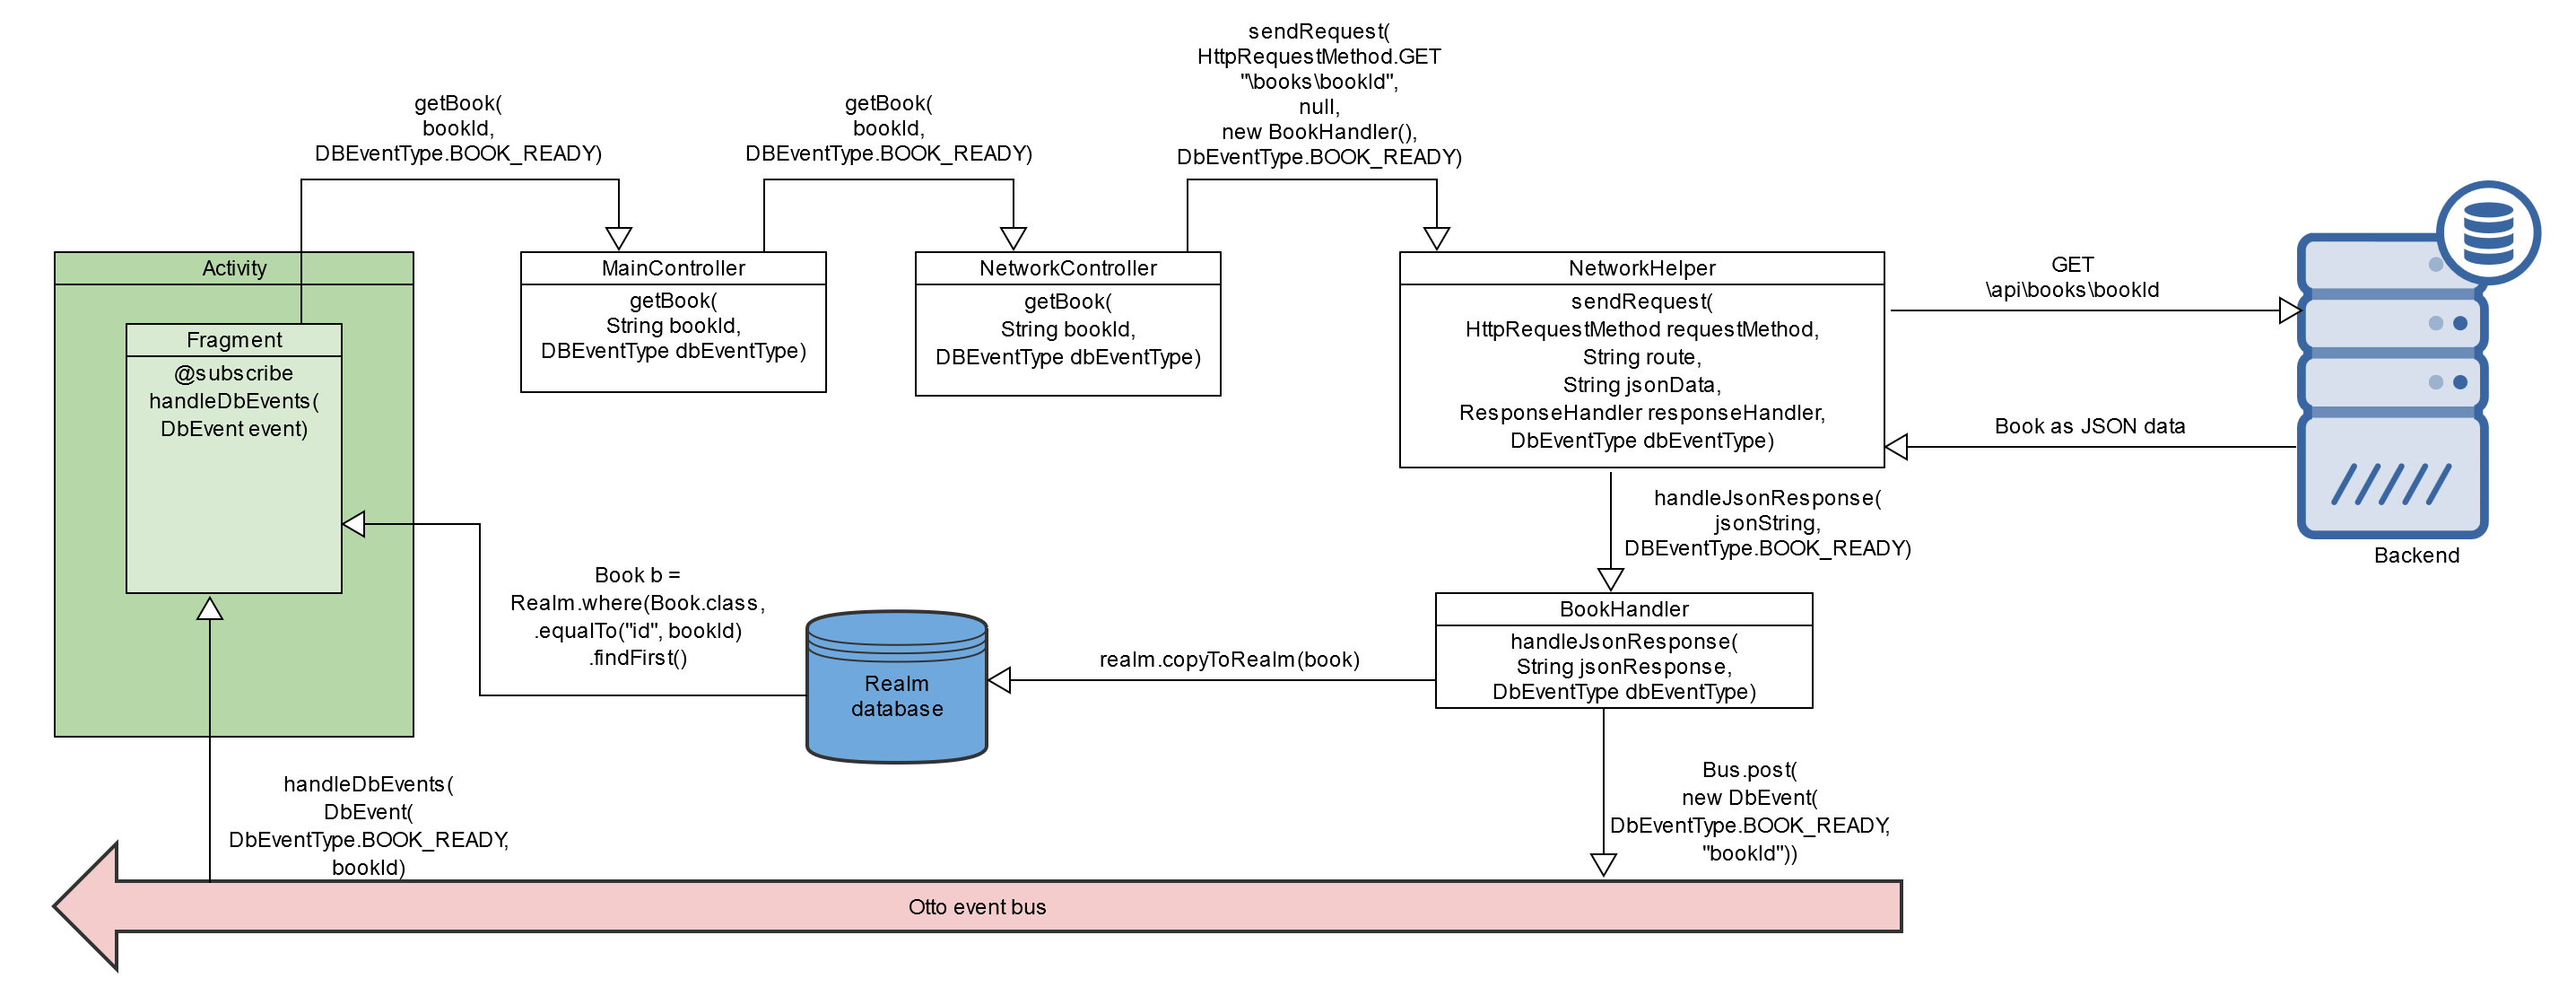
\includegraphics[width=\paperwidth,height=\paperheight,keepaspectratio,angle=90,origin=c]{figs/arch_diagv2.png}
    \caption{How \gls{API} communication and persistent storage works in the Android application}
    \label{fig:Android-api-communication}
\end{figure}

\subsubsection{Important networking files}
    \begin{description}
        \item{\code{HttpRequestMethod.java}} \\
            A simple enum for the POST, PUT, GET and DELETE HTTP request methods.
        \item{\code{Response.java}} \\
            A response-object consists of the received JSON-data, the response-code and reponse message received from server, e.g. "200 OK".
        \item{\code{NetworkController.java}} \\
            Contains one method for each of the functions of the library service API, such as login, getUser and addRenter. The methods constructs a request with the URI for the \gls{API} request, the JSON-data to be sent, if any, and a reponsehandler, if the request should exepect data in return from the library service.   
        \item{\code{NetworkHelper.java}} \\
            Sends a request asynchronously using the specified requestmethod with the specified JSON-data to a specified URI. If the response contains JSON-data, if passes the data along to the specified responsehandler 
        \item{\code{GetBookInfo.java}} \\
            Retrieves meta-information about the given ISBN from the Google Books \gls{API} asynchronously, puts the result in the Realm database and posts an event on the bus when the results is ready. 
        \item{\code{ResponseHandler.java}} \\
            Interface for the responsehandlers. Includes the method handleJsonResponse which all responsehandlers should implement, in addition to a GsonBuilder \cite{gson} with specific settings responsehandlers can use for JSON-data to actual Java objects.
        %\item{Serializers} \\
        %    A Gson-compatible serializer that takes in a Java object and parses it to JSON-data.
    \end{description}

\section{iOS}
\label{architecture-ios}

The iOS application is developed as an native application using the Swift programming language and Apple's Xcode \gls{IDE}.\cite{xcode} The application is based on \gls{MVC}, but with some modifications explained in section \ref{ios-architectural-pattern}.

\subsection{Architectural pattern}
\label{ios-architectural-pattern}
When developing applications for iOS, the view controllers usually become too bloated.\cite{mega-view-controller} They are often a combination of the classic \gls{MVC} controller and additional responsibilities such as responding to user interaction, acting as delegate for contained views, and memory management. Therefore the team decided to use a hybrid architecture, illustrated in figure \ref{fig:ios-mvc-mvvc-model-6}, combining the classical \gls{MVC} and a simple version of the viewmodel from the \gls{MVVM} pattern.\cite{MVVM} This would remove the responsibility of defining the data for views from the view controllers to the viewmodels. Thus reducing their complexity.

\begin{figure}
    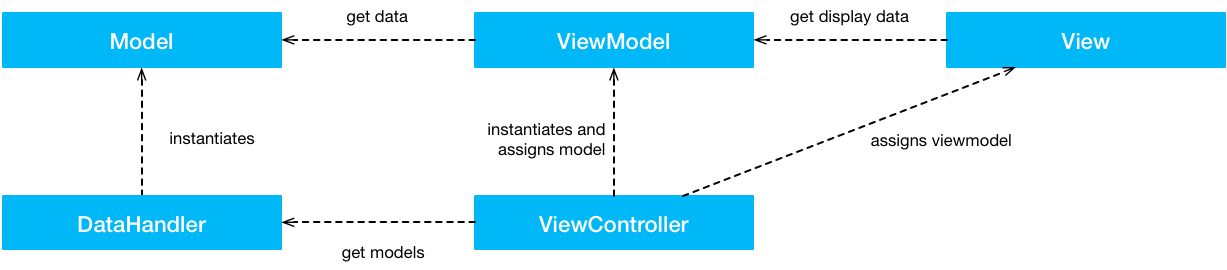
\includegraphics[width=\textwidth,keepaspectratio,origin=c]{figs/v06/iOS/mvc-mvvm-model.png}
    \caption{Diagram that shows how the combination of \gls{MVC} and \gls{MVVM} works in the iOS application}
    \label{fig:ios-mvc-mvvc-model-6}
\end{figure}

\subsection{Structure}
As previously stated, the iOS application is heavily based on the \gls{MVC} architectural pattern. This entails that the system is relatively modularized and loose coupled. Figure \ref{fig:ios-shelf-class-diagram-6} and \ref{fig:ios-book-view-class-diagram-6}  illustrates how parts of the system is structured. 

The \code{DataHandler} is located at the bottom of the diagrams. This acts as a broker by abstracting the process of selecting endpoints and structuring requests in order to keep the business logic as clean as possible.\cite{progark} All data returned from the \code{DataHandler} class is represented as models. The models are created using a factory method that instantiates a new model object and populates it using a provided \gls{JSON} object.\cite{progark}

The view controller requests data from the \code{DataHandler}, and presents it to the user. If data should be structured in lists or grids, this is achieved  of through the delegate pattern combined with Apple's UIKit.\cite{progark}\cite{uikit} In order to respond to updates such as the users authentication state, the publish-subscribe patterns is used to send notifications.\cite{progark}

Because all the views in the application were made using Xcode's interface builder, and view controllers acts like a combination of views and controllers, there are few dedicated view classes. A couple of exceptions are table view cells and grid views, which are implemented using  viewmodels for presenting data.

\begin{figure}
    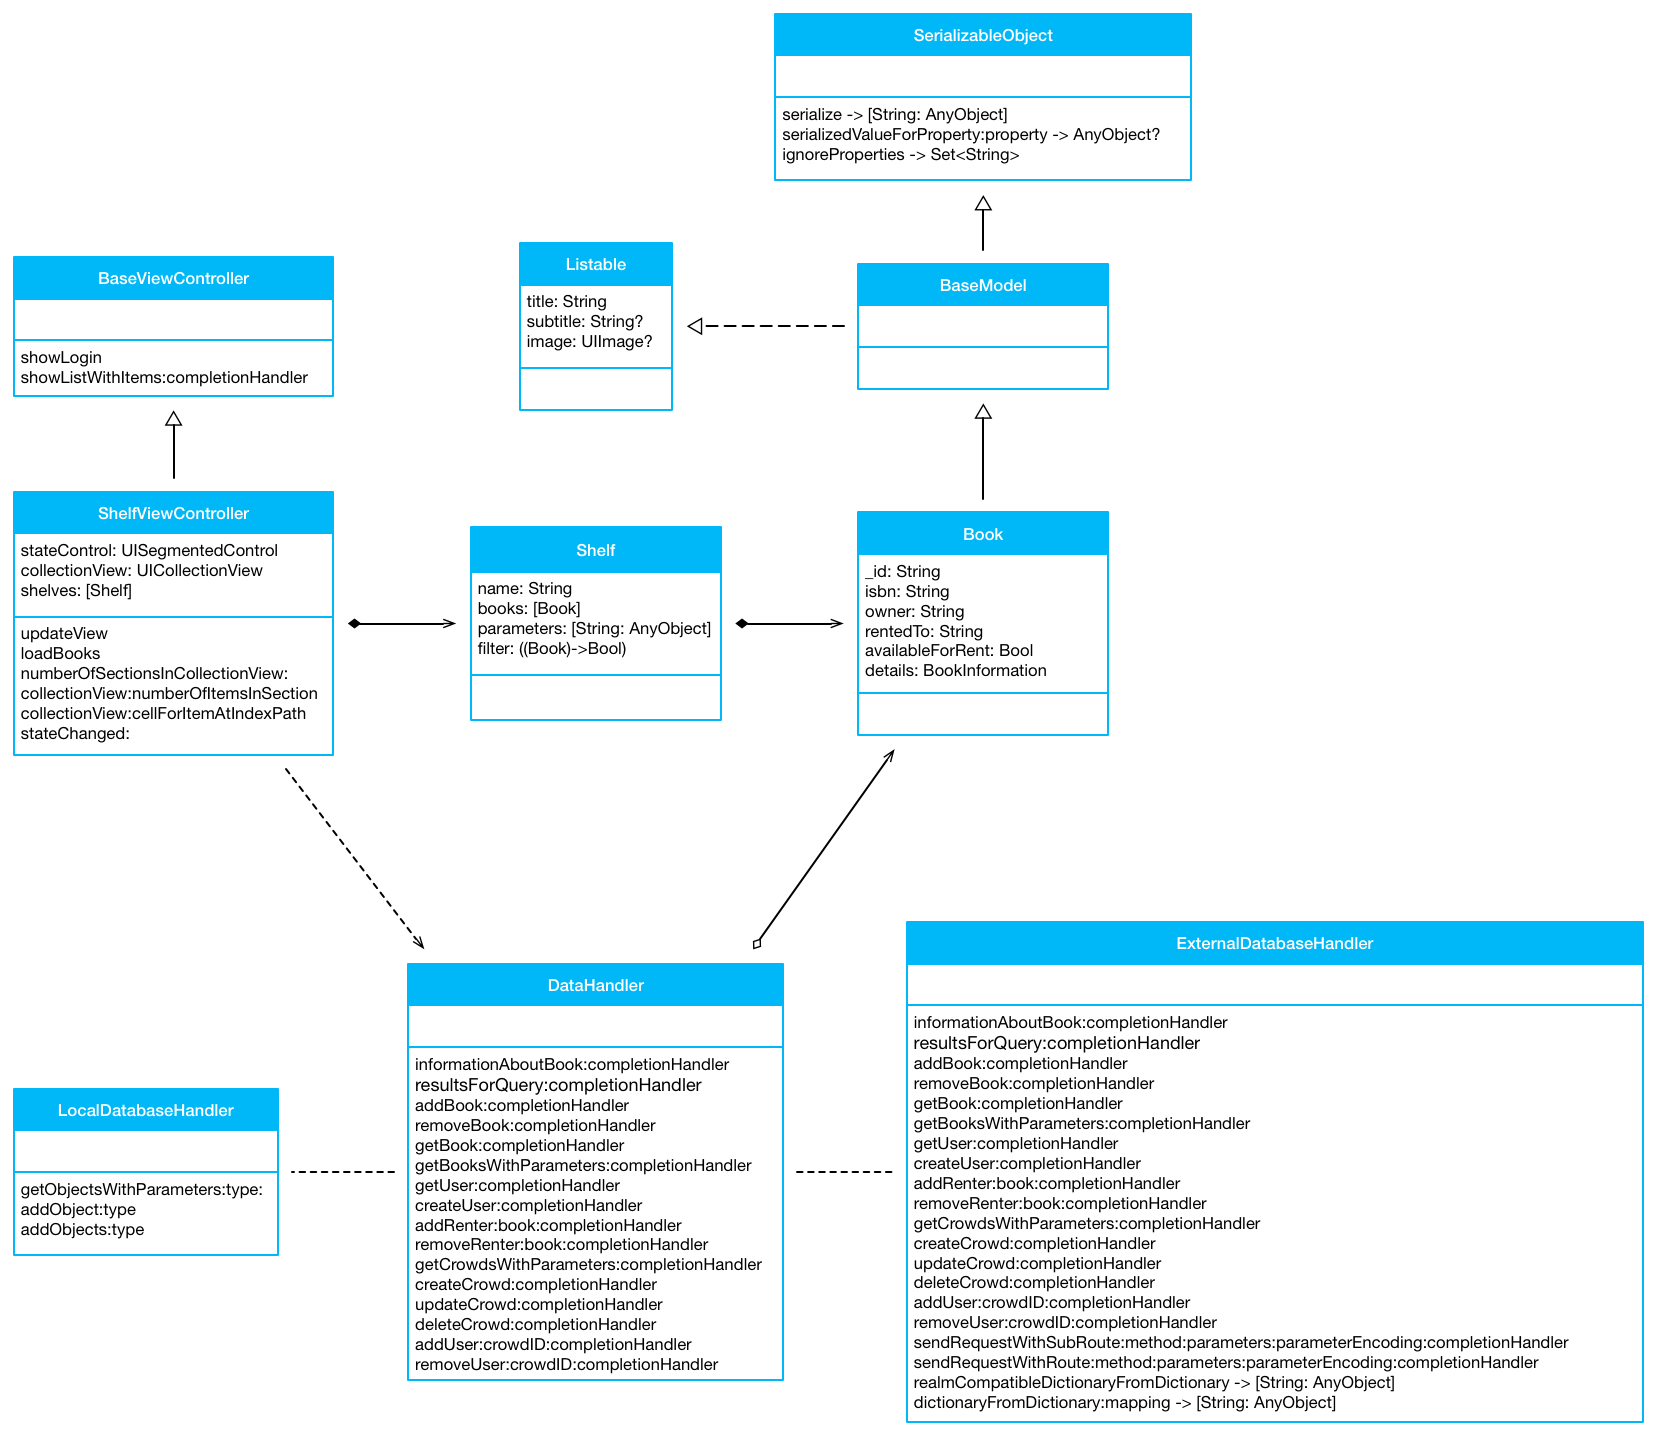
\includegraphics[width=\textwidth,keepaspectratio,origin=c]{figs/v06/iOS/shelf-class-diagram.png}
    \caption{A fragment of the class diagram showing how components related to the shelf view are connected}
    \label{fig:ios-shelf-class-diagram-6}
\end{figure}

\begin{figure}
    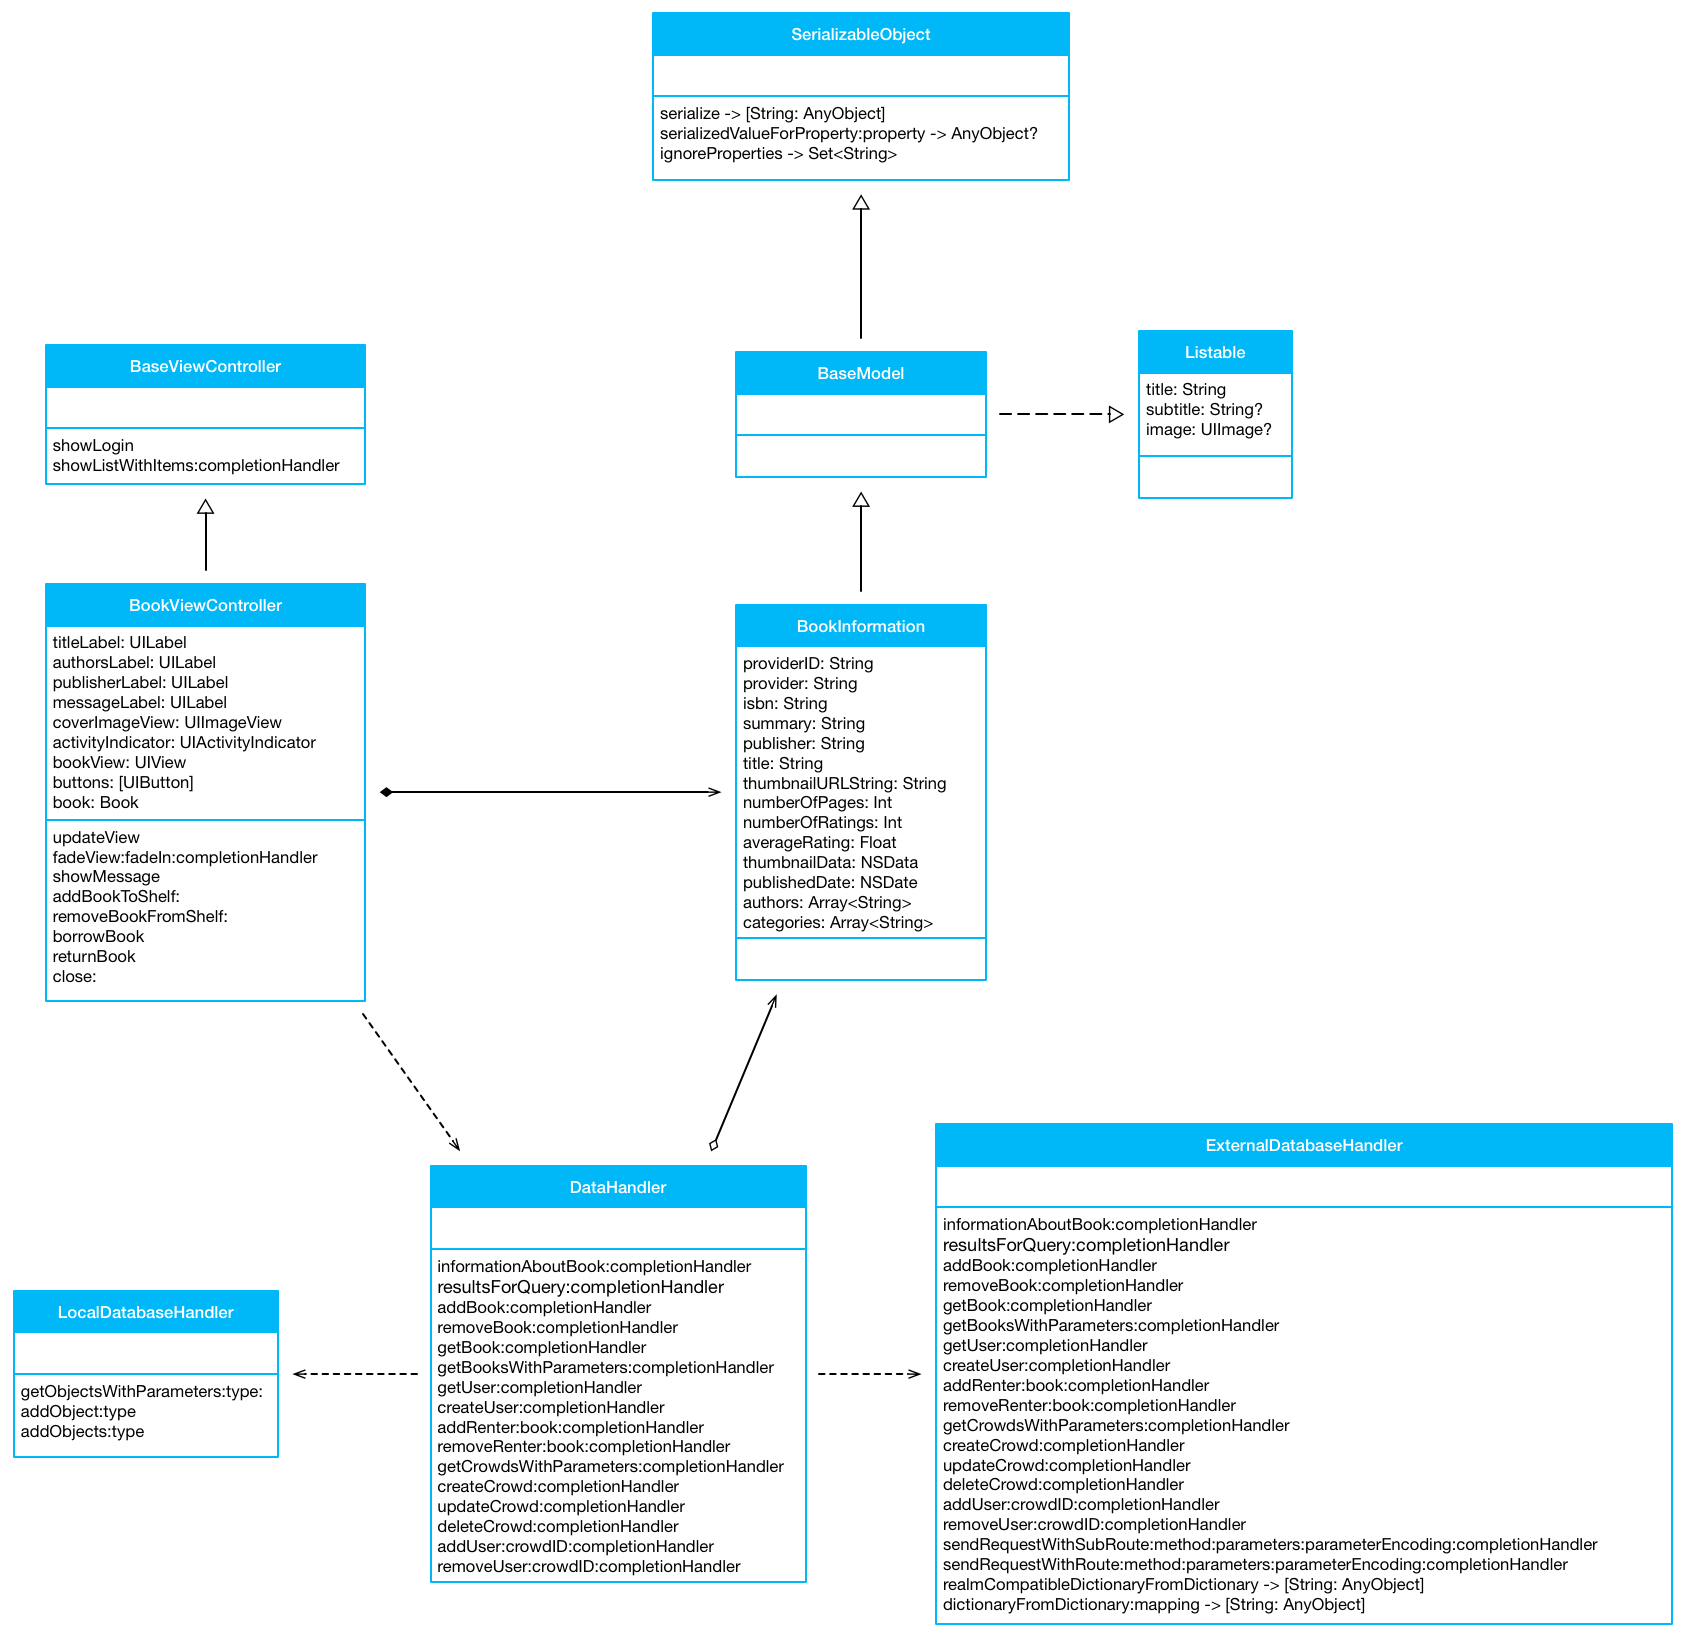
\includegraphics[width=\textwidth,keepaspectratio,origin=c]{figs/v06/iOS/book-view-class-diagram.png}
    \caption{A fragment of the class diagram showing how components related to the book view are connected}
    \label{fig:ios-book-view-class-diagram-6}
\end{figure}


\subsection{Network, \gls{API} and storage}
Because the application operates using both local and external data, it is important to design data operations to be as efficient as possible given the response time and availability issues a network request imposes. 

The iOS teams approach to the problem is that every time data is requested, a premature callback is sent with the data from cache, as illustrated in figure \ref{fig:ios-get-request-process-6}. This ensures that the perceived response time is shorter than the actual response time. The solution could lead to some issues if the external response is delayed, and the user tries to update old data. When the \gls{HTTP} response is received, the data updated data is stored in the local database and returned with a second callback call.

\begin{figure}
    \includegraphics[width=\textwidth,keepaspectratio,origin=c]{figs/v06/iOS/get-request-sequence-diagram.png}
    \caption{Diagram that shows how a GET request is processed in the iOS application}
    \label{fig:ios-get-request-process-6}
\end{figure}

When the application tries to update some data, the external request is sent first, as illustrated in figure \ref{fig:ios-put-request-process-6}. If the request is successful, the local database is updated as well. This ensures that the local database is synchronized with the external database.

\begin{figure}
    \includegraphics[width=\textwidth,keepaspectratio,origin=c]{figs/v06/iOS/put-request-sequence-diagram.png}
    \caption{Diagram that shows how a PUT request is processed in the iOS application}
    \label{fig:ios-put-request-process-6}
\end{figure}